\section{Introduzione}

\begin{domanda}
    (Cosa signifca costruire un classificatore?)

    Significa costruire una superficie di separazione. Per farlo si allena un
    modello utilizzando dei dati etichettati, che prende il nome di
    \textbf{training set}. Le superfici di separazione ci aiutano a classificare
    nuovi dati non visti.

    \textit{Esempio semplice}: chi paga il mutuo e chi no.
\end{domanda}

Una superficie di separazione è definita come:

$$ H(v,\gamma) = \{x \in \mathcal{R}^n | v^T x = \gamma\} $$
con:
\begin{itemize}
    \item $v \in R^n$ è un vettore, chiamato $normale$
    \item $\gamma \in R$ è uno scalare, che è il $bias$
\end{itemize}

La funzione \textbf{sign} ci dice da che parte del piano si trova un punto.
Cioè, dato un punto $\bar{x}$, se $sign(v^T \bar{x} - \gamma) \geq 0$ allora è
un cliente che paga il mutuo, altrimenti no.

\begin{domanda}
    (Dove interviene l'ottimizzazione quando si costruisce un classificatore? Perché serve?)

    Il classificatore viene costruito andando a \textbf{minimizzara} una misura che
    indica quanto si sta sbagliando nel classificare i punti.
\end{domanda}

\section{Programmazione non lineare}

\begin{definition}
    (Minimo globale)
    Dato un punto $x^* \in R^n$ si dice minimo globale se:
    \begin{itemize}
        \item $x^* \in X$, cioè il punto appartiene alla \textbf{regione ammissibile}
        \item $f(x^*) \leq f(x \forall x \in X)$, cioè per ogni punto della regione ammissibile, il valore di funzione obiettivo su $x^*$ è minore uguale rispetto agli altri punti.
    \end{itemize}
\end{definition}

\textbf{Notina:} Definizione di programma lineare:

\begin{itemize}
    \item $f(x) = c^T x$
    \item $X = \{x \in R^n | Ax = b, x \geq 0\}$
\end{itemize}
Dove $X$ è la regione ammissibile ed è un $poliedro$.

\begin{definition}
    (Minimo locale)

    Un punto $x^* \in X$ è un minimo locale per il problema $P$ se:
    \begin{itemize}
        \item $x^* \in X$
        \item Esiste un vicinato $N$ tale che $f(x^*) \leq f(x) \forall x \in X \cap N$. Cioé
              ogni punto della regione ammissibile intersecato col vicinato, e il valore
              $x^*$ è sempre minore.
    \end{itemize}
\end{definition}

Il vicinato è un insieme di punti, non so come definito ma ok.

\

\begin{definition}
    (Minimo locale stretto)

    Un punto $x^* \in X$ è un minimo locale stretto per il problema $P$ se:
    \begin{itemize}
        \item $x^* \in X$
        \item Esiste un vicinato $N$ tale che $f(x^*) < f(x) \forall x \neq x^*, x \in X \cap
                  N$.
    \end{itemize}
    Spiegazione al volo: Il minimo locale stretto è un minimo locale, ma non esistono altri punti che hanno lo stesso valore di funzione obiettivo.

    \begin{figure}[H]
        \centering
        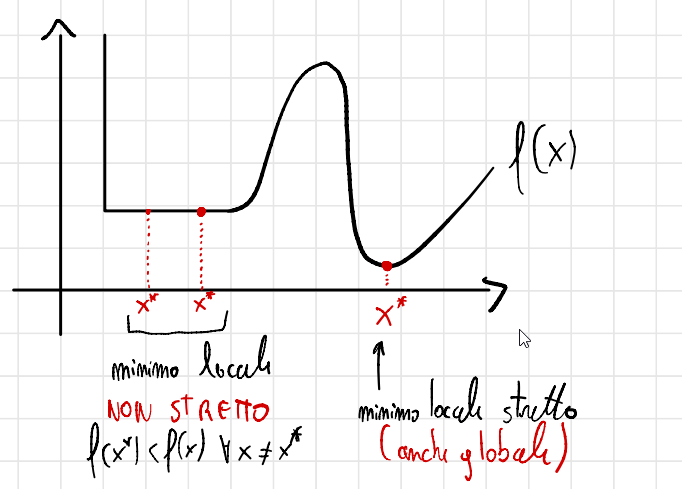
\includegraphics[width=0.8\textwidth]{images/minimo locale.png}
        \caption{Esempio di minimo locale stretto}
        \label{fig:esempio-di-minimo-locale-stretto}
    \end{figure}
\end{definition}

\textbf{Nota:} Se $x^*$ è un minomo globale implica che $x^*$ è un minimo locale.

\begin{definition}
    (Combinazione convessa)

    Dati $x^{(1)}$ e $x^{(2)}$ due punti $\in R^n$, la combinazione convessa di
    $x^{(1)}$ e $x^{(2)}$ è un vettore:

    $$
        \bar{x} = \lambda x^{(1)} + (1 - \lambda) x^{(2)}$$
    con $\lambda \in [0,1]$

    Immagina una retta che unisce i due punti, con $\lambda$ = 0 in $x^{(1)}$ e
    $\lambda$ = 1 in $x^{(2)}$.
\end{definition}

\begin{definition}
    (Funzione convessa)

    Data una funzione $f: R^n \rightarrow R$, $f$ è \textbf{convessa} se per ogni
    coppia di punti $x^{(1)}, x^{(2)} \in R^n$ e per ogni $\lambda \in [0,1]$ vale
    che: $$ f(\lambda x^{(1)} + (1 - \lambda) x^{(2)}) \leq \lambda f(x^{(1)}) + (1
        - \lambda) f(x^{(2)}) $$

    Cioè in italiano, il valore di funzione della combinazione dei due vettori è
    minore o uguale alla combinazione dei valori di funzione dei due vettori.

    \begin{figure}[H]
        \centering
        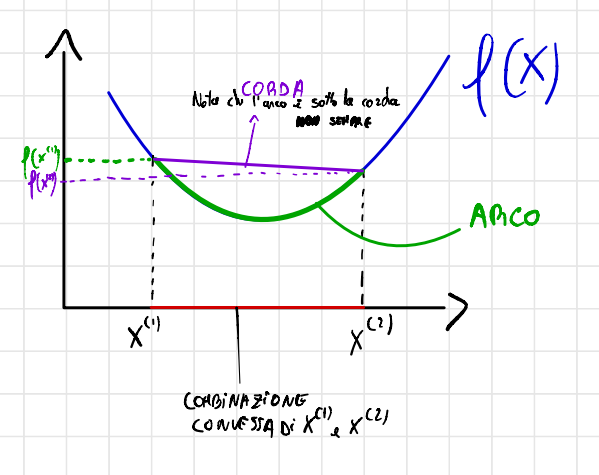
\includegraphics[width=0.8\textwidth]{images/funz conv.png}
        \caption{Esempio di funzione convessa}
        \label{fig:esempio-di-funzione-convessa}
    \end{figure}

    \begin{figure}[H]
        \centering
        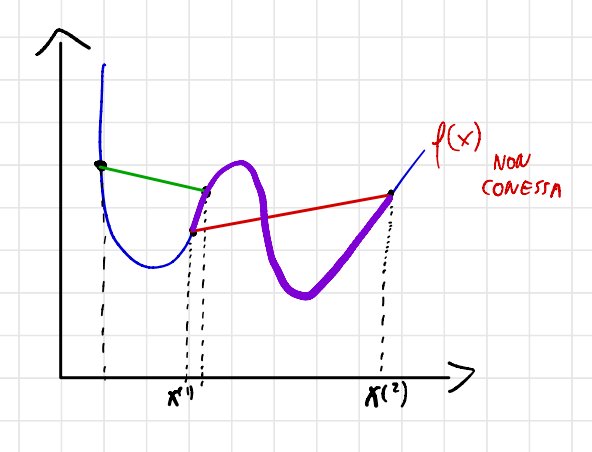
\includegraphics[width=0.8\textwidth]{images/non conv.png}
        \caption{Esempio di funzione non convessa}
        \label{fig:esempio-di-funzione-non-convessa}
    \end{figure}

    Per capire, diciamo che la funzione è convessa se per ogni valore di funzione
    su un punto che è all'interno della combinazione convessa dei due punti, il
    valore di funzione è minore o uguale alla combinazione dei valori di funzione
    dei due punti.

    Infatti, nel secondo esempio, ci sono dei punti tali per cui la funzione è
    maggiore (cioè sta sopra).
\end{definition}

\begin{domanda}
    (Quando un punto di un'insieme convesso è estremo?)

    $\bar{x} \in X$ è un punto estremo di un'insieme convesso se NON ESISTE nessuna coppia di punti $x^{(1)}, x^{(2)} \in X$ e $\lambda \in (0,1)$ tale che:
    $\bar{x} = \lambda x^{(1)} + (1 - \lambda) x^{(2)}$, per $\lambda \in ]0,1[$.

    Banalmente, un punto è estremo se non è combinazione convessa di altri punti.
\end{domanda}

\textbf{Nota:} $P$ è un programma convesso se $f$ è una funzioen convessa e $X$ è un'insieme convesso. Questo ci serve saperlo perché in caso di
\textbf{programma convesso} abbiamo che il minimo globale e locale \textbf{coincidono}.

\begin{domanda}
    (Cosa cerchiamo con un problema di ottimizzazione?)

    Cerchiamo il \textbf{minimo locale}, perché cercare il minimo globale fa parte
    di un'altra categoria di problemi, che sono quelli di \textbf{ottimizzazione
        globale}.
\end{domanda}

\subsubsection{Caso di problemi senza vincoli}

In questo caso, la regione ammissibile $X$ coincide con $R^n$.

$$
    P = \begin{cases}
        \min f(x) \\
        f(x): \mathcal{R}^n \rightarrow R
    \end{cases}
$$

\textbf{Nota:} Si fa un'assunzione. $f \in C^2$, cioè la funzioen è due volte
continuamente differenziabile. Quindi, $C^2$ è l'insieme di funzioni che ammettono prima e seconda derivate continue.

Questa assunzione ci permette di dire che $\bar{x} \in R^n \implies \nabla f(\bar{x})$ e $\nabla^2 f(\bar{x})$ esistono.


Vediamo come si applica il gradiente e la matrice hessiana.

\begin{definition}
    (Gradiente)

    Il gradiente di una funzione $f: R^n \rightarrow R$ è un vettore di dimensione
    $n$ che contiene le derivate parziali della funzione rispetto alle sue
    variabili.

    $$
        \nabla f(x) = \begin{bmatrix}
            \frac{\partial f}{\partial x_1} \\
            \frac{\partial f}{\partial x_2} \\
            \vdots                             \\
            \frac{\partial f}{\partial x_n}
        \end{bmatrix}
    $$
\end{definition}

\begin{definition}
    (Matrice Hessiana)

    La matrice hessiana di una funzione $f: R^n \rightarrow R$ è una matrice
    quadrata di dimensione $n$ che contiene le derivate seconde parziali della
    funzione rispetto alle sue variabili.

    $$
        \nabla^2 f(x) = \begin{bmatrix}
            \frac{\partial^2 f}{\partial x_1^2} & \frac{\partial^2 f}{\partial x_1 \partial x_2} & \dots  & \frac{\partial^2 f}{\partial x_1 \partial x_n} \\
            \frac{\partial^2 f}{\partial x_2 \partial x_1} & \frac{\partial^2 f}{\partial x_2^2} & \dots  & \frac{\partial^2 f}{\partial x_2 \partial x_n} \\
            \vdots & \vdots & \ddots & \vdots \\
            \frac{\partial^2 f}{\partial x_n \partial x_1} & \frac{\partial^2 f}{\partial x_n \partial x_2} & \dots  & \frac{\partial^2 f}{\partial x_n^2}
        \end{bmatrix}
    $$
\end{definition}

\begin{esempio}
    f(x) = $8x_1 + 12x_2 + x_1^2 - 2x_2^2$

    Iniziamo dal gradiente.

    $$
        \nabla f(x) = \begin{bmatrix}
            8 +2x_1 \\
            12 - 4x_2
        \end{bmatrix}
    $$

    Ora la matrice hessiana.

    $$
        \nabla^2 f(x) = \begin{bmatrix}
            2 & 0  \\
            0 & -4
        \end{bmatrix}
    $$
    
    Dando un valore ad $x$, ad esempio $x = \begin{bmatrix}
        1 \\
        1
    \end{bmatrix}$, possiamo calcolare il gradiente e la matrice hessiana cosi:

    $$
        \nabla f(x) = \begin{bmatrix}
            10 \\
            8
        \end{bmatrix}
    $$

    $$
        \nabla^2 f(x) = \begin{bmatrix}
            2 & 0  \\
            0 & -4
        \end{bmatrix}
    $$
\end{esempio}


\section{Approcci di classificazione}
\label{sec:approcci-di-classificazione}

Abbiamo diversi approcci di classificazione.

\begin{itemize}
    \item \textbf{Supervised learning}: Abbiamo un'insieme di dati che sono \textbf{etichettati}.
          Questo rappresenta il nostro \textbf{training set}. Il nostro obiettivo è fare
          predizioni sulle etichette di dati non ancora visti. Le etichette rappresentano
          la \textbf{classe}.
    \item \textbf{Unsupervised Learning}: I dati non hanno alcuna etichetta. Il nostro
          obiettivo è fare operazioni di \textbf{clustering}, ovvero raggruppare i dati in base a quanto sono simili tra loro.
    \item \textbf{Semisupervised Learning}: Abbiamo entrambi i tipi di dati (con e senza etichette). L'obiettivo è predirre la label
          dei dati non etichettati.
\end{itemize}

Il modo in cui chiamo i dati all'interno del nostro dataset sono molteplici,
tipo:
\begin{enumerate}
    \item Datum
    \item Object
    \item Feature Vectore / Vettore delle caratteristiche
    \item Punto
\end{enumerate}

\begin{definition}
    (Classifier)

    Un classificatore è una \textbf{superficie di separazione} tra le classi.
\end{definition}
\newpage
\section{Separazione Lineare}
\begin{definition}
    (Separazione Lineare)
    Dati due insiemi $A = \{a_1, a_2, \dots, \_m\}$ e $B = \{b_1, b_2, \dots, b_k\}$. Due insiemi si dicono \textbf{linearmente separabili} $\iff$ esiste un iperpiano $H(v,\gamma)$ che separa i due insiemi.

    $$
        H(v,\gamma) = \{x \in \mathcal{R}^n | v^T x = \gamma\}
    $$
    con:
    \begin{itemize}
        \item $v \in R^n$ è un vettore
        \item $\gamma \in R$ è uno scalare
        \item $v \neq 0$
    \end{itemize}

    Questo iperpiano, tale che:

    $$
        v^T a_i \geq \gamma + 1 \land v^T b_j \leq \gamma - 1
    $$
    per $i = 1, \dots, m$ e $j = 1, \dots, k$.
\end{definition}

\textbf{Nota e possibile domanda}: Quando andiamo a classificare non teniamo conto del +1 e -1, perché vengono usati solo per costruzione.
Quindi la disequazione conta solamente il valore di $\gamma$ (nel lato desto).

\textbf{Nota 2:} I due insiemi $A$ e $B$ sono linearmente separabili $\iff$ \textbf{l'intersezione} della loro copertura convessa è vuota.
$$
    conv(A) \cap conv(B) = \emptyset
$$

\begin{definition}
    (Copertura Convessa)

    La copertura convessa di un'insieme $X$ è l'insieme convesso più piccolo che lo
    contiene.

    Un'insieme si dice convesso se per ogni coppia di punti $(x,y) \in X$ la
    combinazione di $x$ e $y$ è sempre all'interno dell'insieme $X$. Formalmente:
    $$ \forall x,y \in X, \forall \lambda \in [0,1] \implies \lambda x + (1 -
        \lambda) y \in X $$
\end{definition}

Implicazione ovvia, ma la copertura convessa di un'insieme convesso è l'insieme
stesso. $ X\ convesso \implies conv(X) = X $

\begin{definition}
    (Funzione Errore | Loss Function)

    Un punto $a_i \in A$ è \textbf{classificato correttamente} se $$ v^T a_i \geq
        \gamma + 1 \implies v^T a_i - \gamma - 1 \geq 0 $$ Questo implica che $a_i$ è
    \textbf{classificato erroneamente} se $$ v^T a_i - \gamma -1 < 0 \implies -v^T
        a_i + \gamma + 1 > 0 $$

    L'errore di $a_i$ è dato da: $$ \max\{0, -v^T a_i + \gamma + 1\} \geq 0 $$

    Analogamente, un punto $b_j \in B$ è \textbf{classificato correttamente} se $$
        v^T b_j - \gamma + 1 \leq 0 $$. Questo implica che $b_j$ è \textbf{classificato
        erroneamente} se $$ v^T b_j - \gamma + 1 > 0 $$

    L'errore di $b_j$ è dato da: $$ \max\{0, v^T b_j - \gamma + 1\} \geq 0 $$
\end{definition}
